\documentclass[../main.tex]{subfiles}

\usepackage{graphicx} % Needed to include images
\usepackage{setspace} % Needed to set spacing

\begin{document}

\chapter{Appendix}
\section{Screenshots of the GUI}

\subsection{3D Shape Configuration and Visualization}
\begin{figure}[H]
\centering
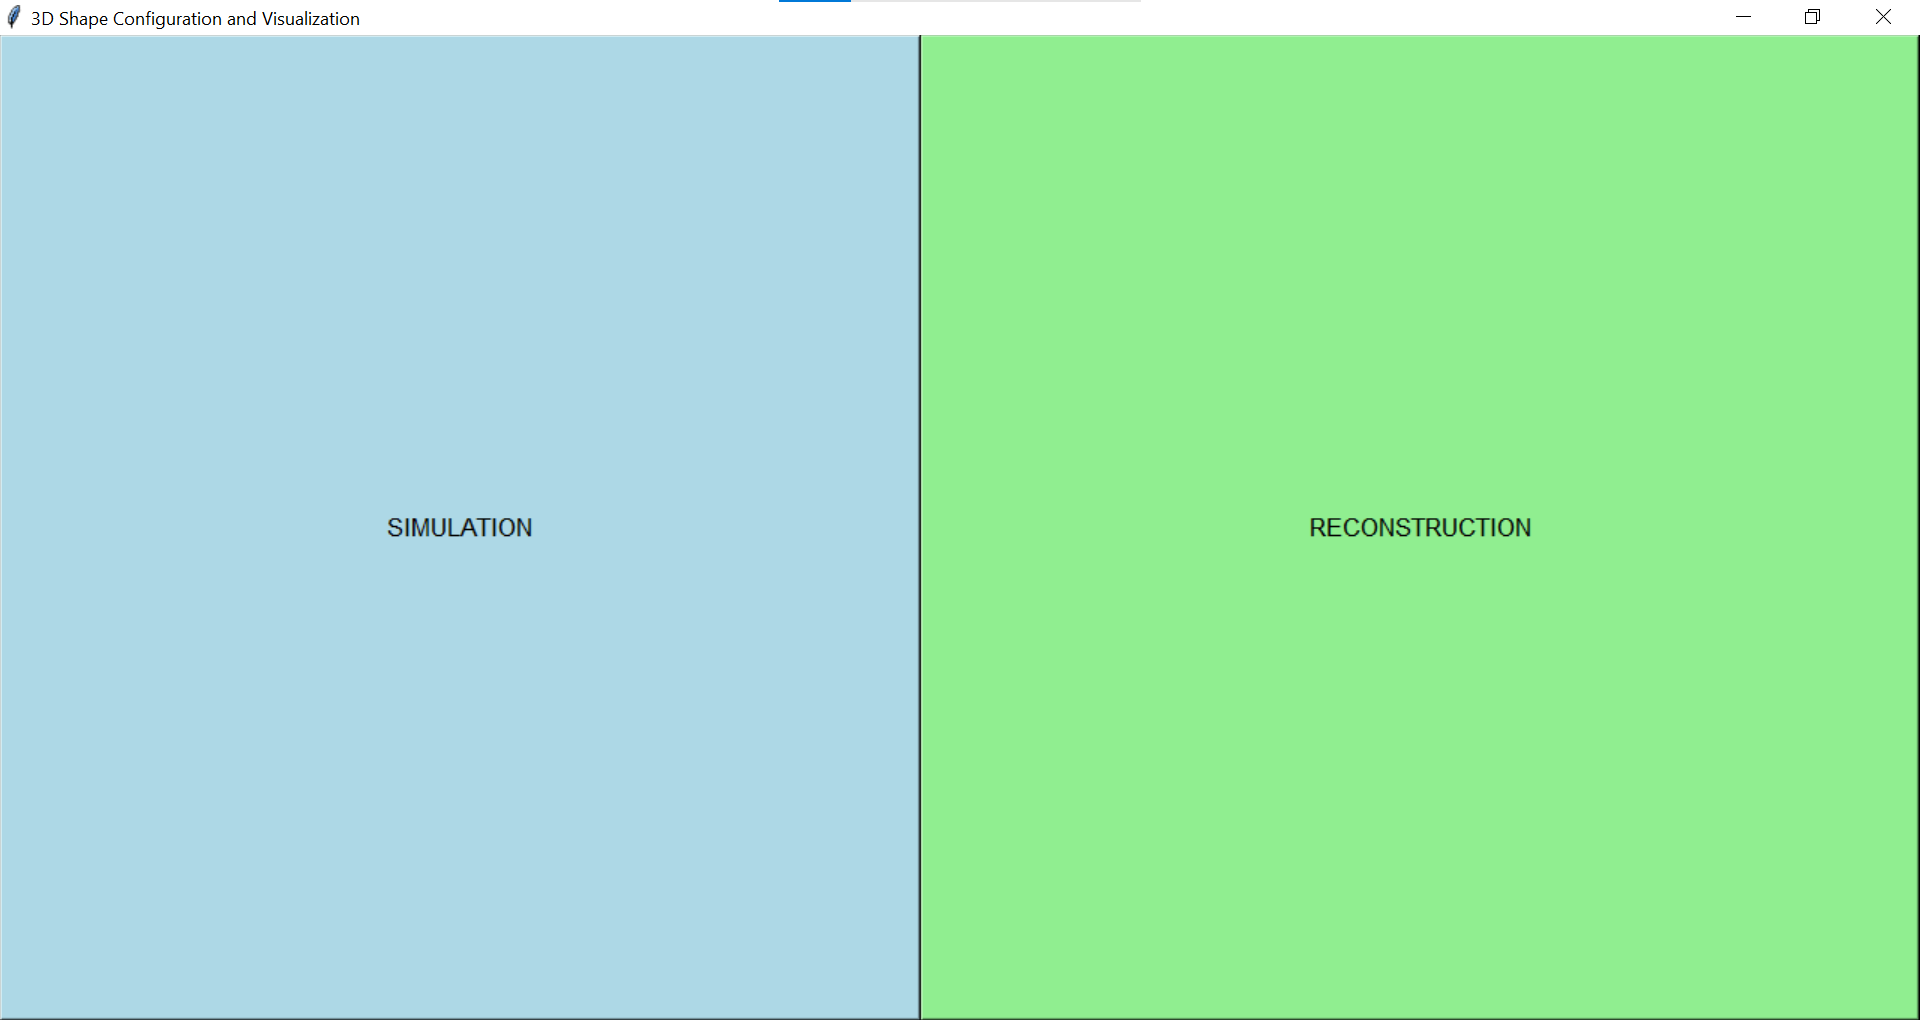
\includegraphics[width=\textwidth]{Images/Appendix/main}
\caption{Initial interface showing two divided sections for simulation and reconstruction processes in the 3D Shape Configuration and Visualization tool.}
\end{figure}

\subsection{Simulation Window - Insert Cylinder}
\begin{figure}[H]
\centering
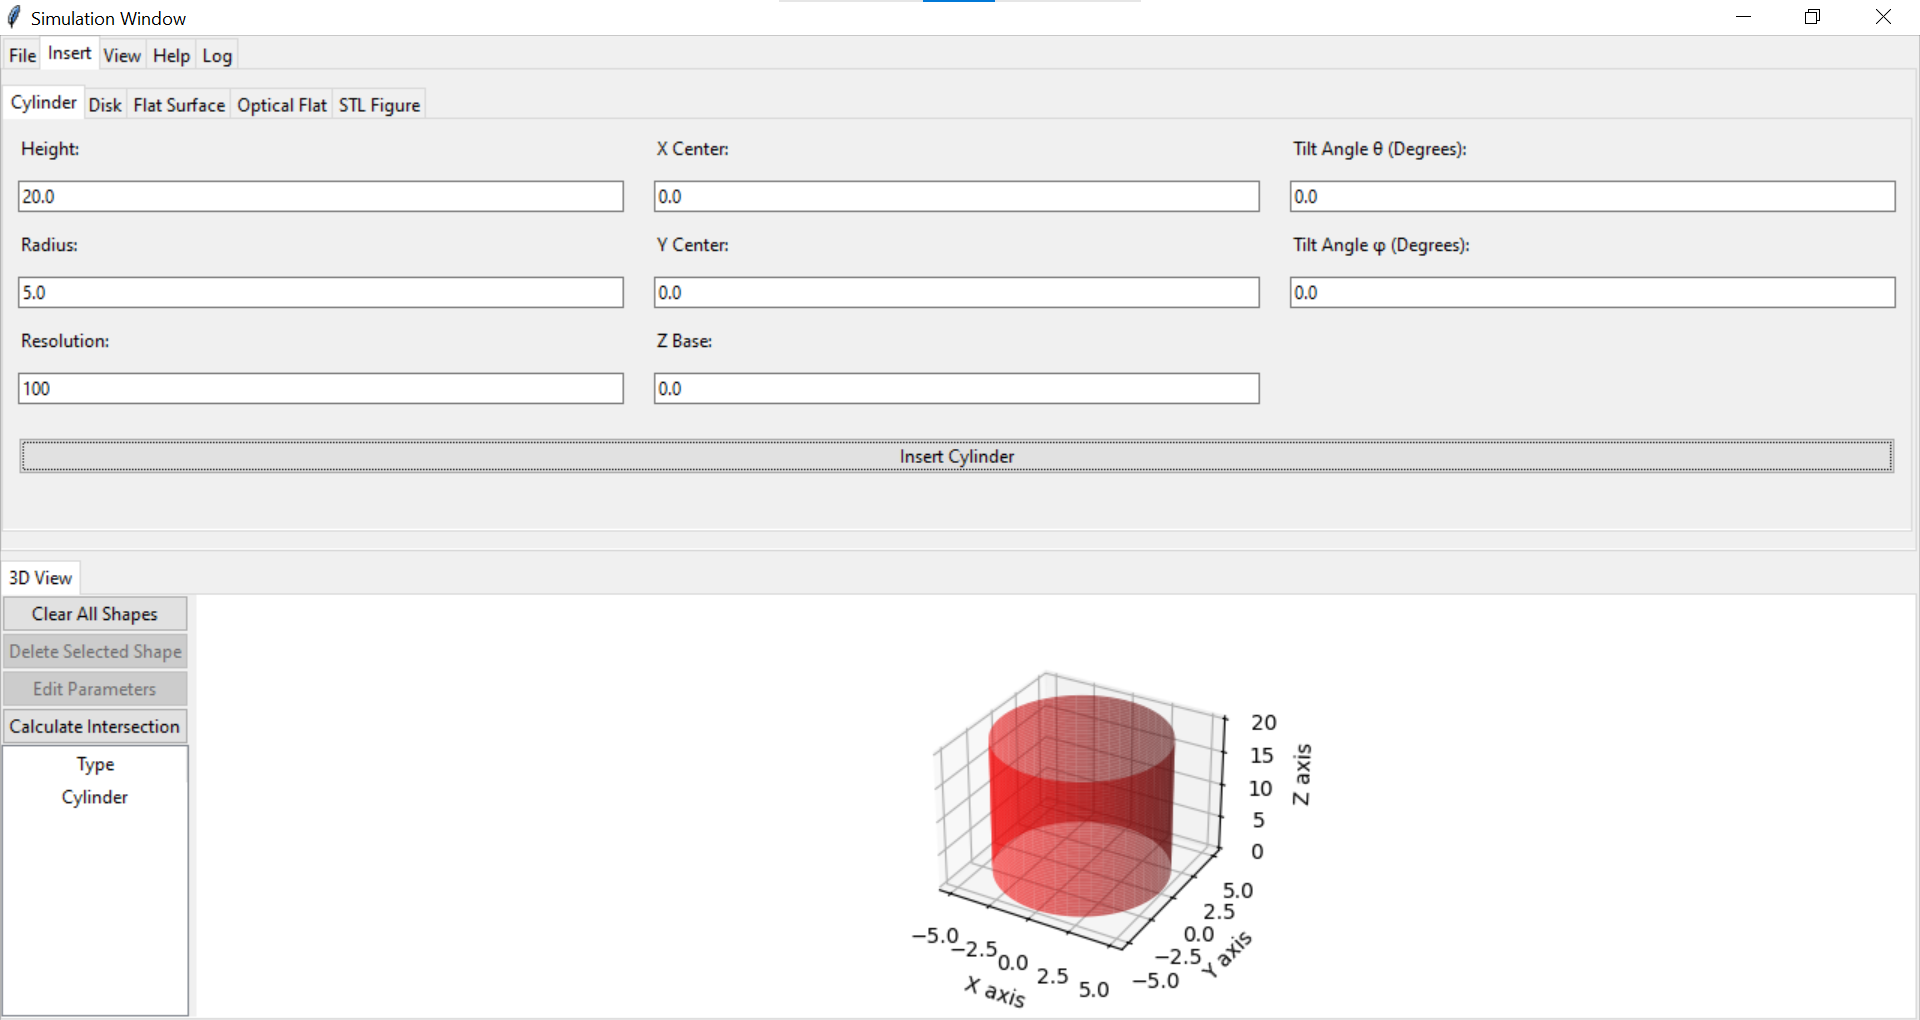
\includegraphics[width=\textwidth]{Images/Appendix/simulation/cylinder}
\caption{Simulation window displaying the parameters for inserting a cylinder and a 3D view of the inserted cylinder with default orientation.}
\end{figure}

\subsection{Cylinder and Optical Flat Intersection}
\begin{figure}[H]
\centering
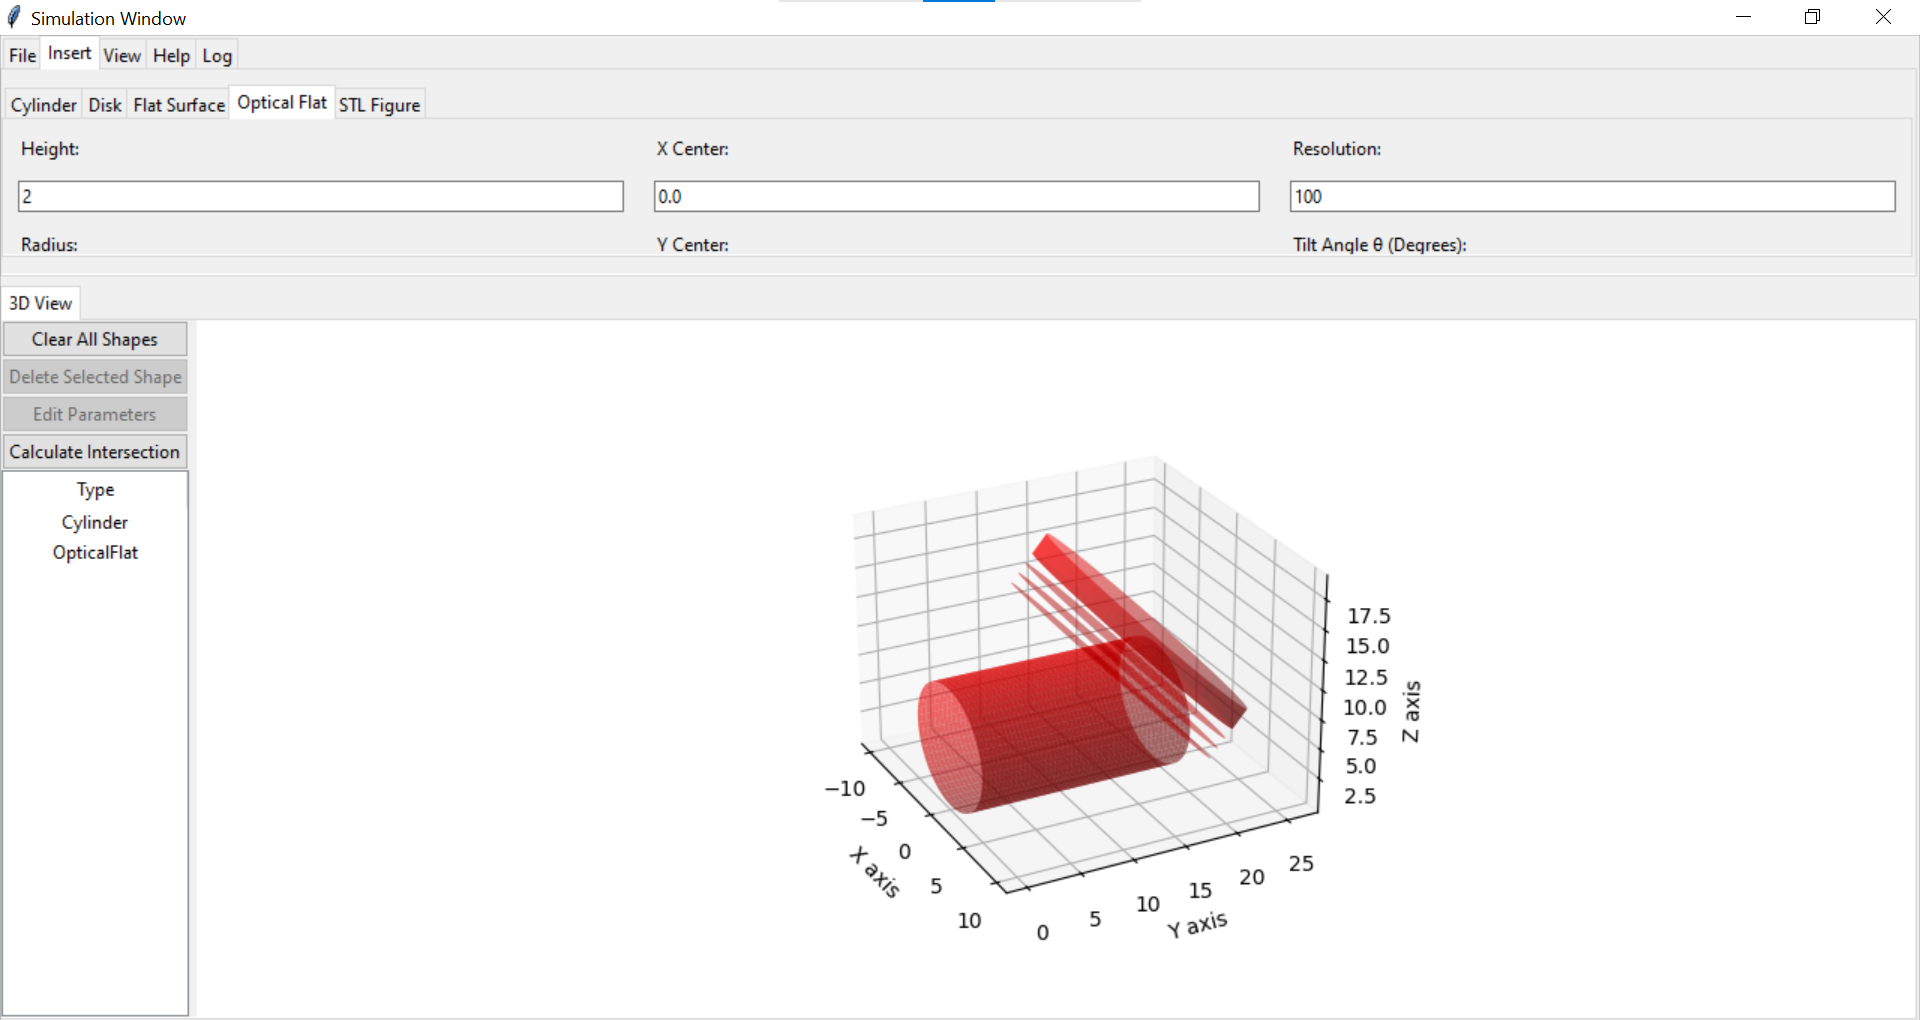
\includegraphics[width=\textwidth]{Images/Appendix/simulation/cylinder_optical_flatr}
\caption{Demonstration of a cylinder intersecting with an optical flat at an angle, visualized in the simulation window.}
\end{figure}

\subsection{Updated Cylinder Position}
\begin{figure}[H]
\centering
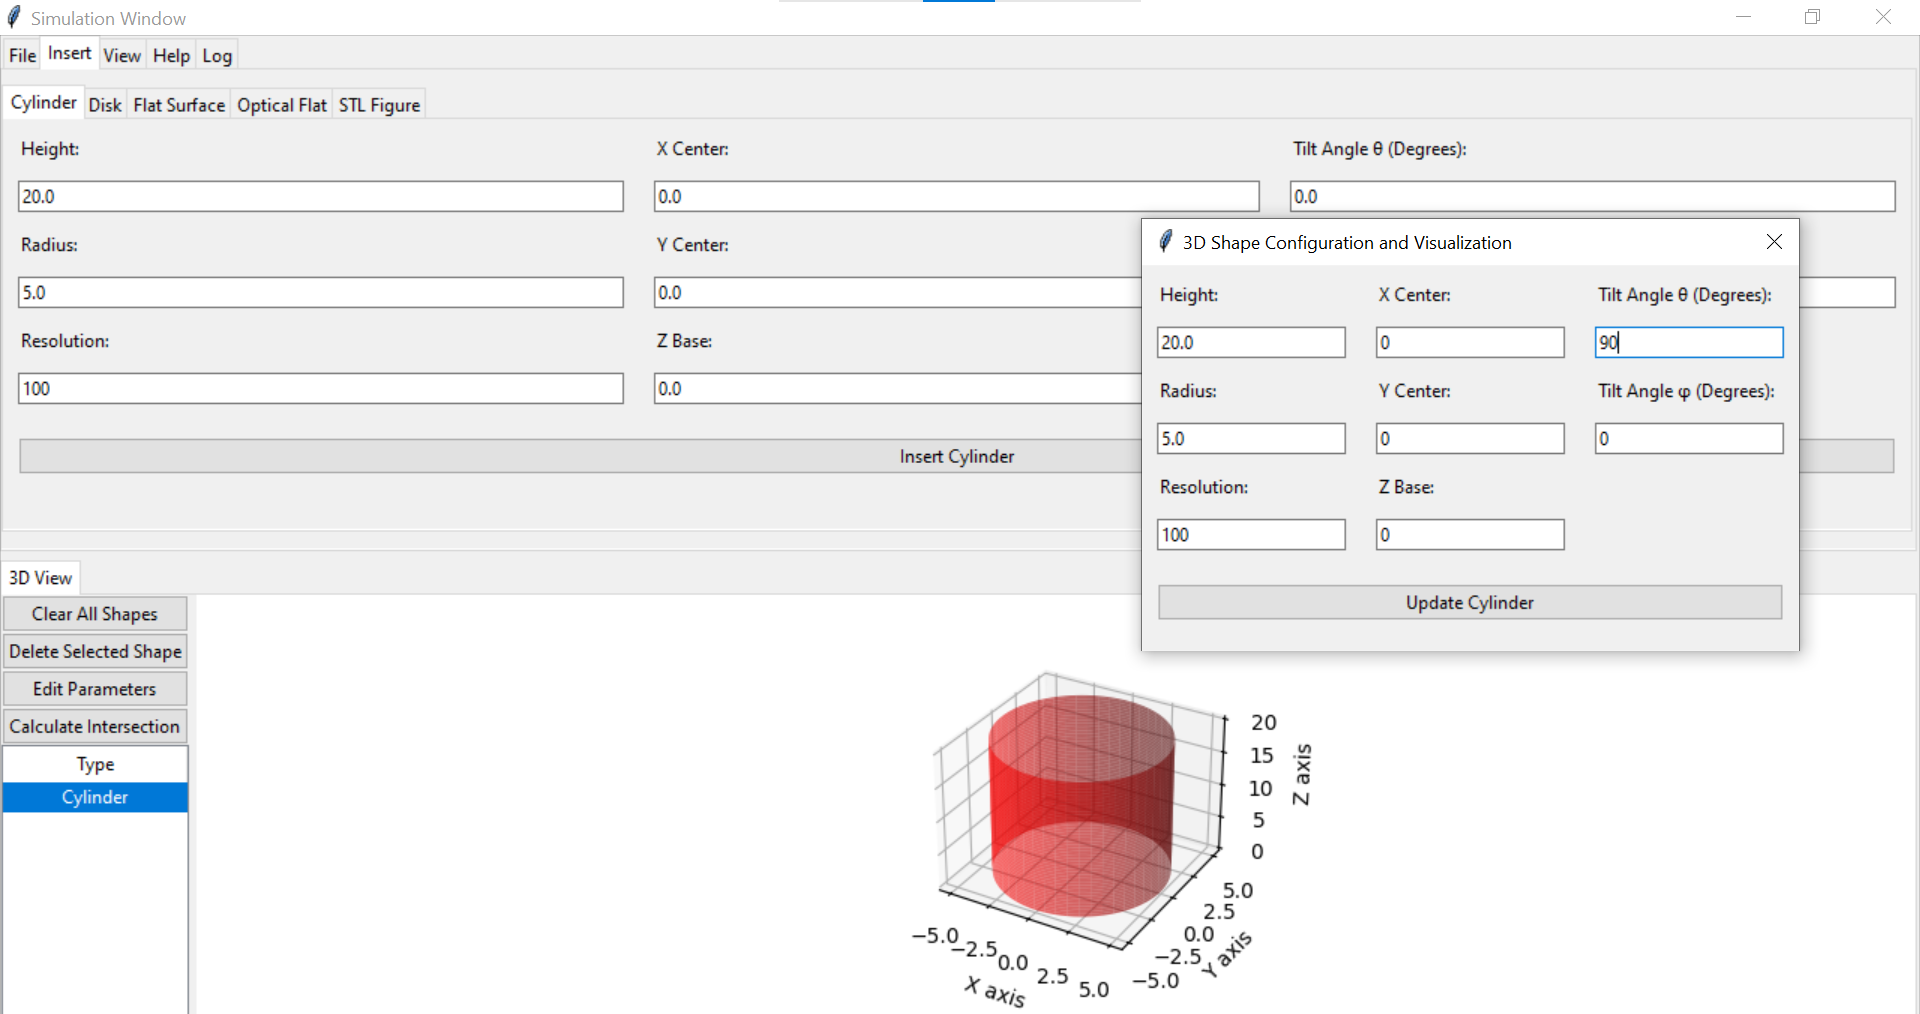
\includegraphics[width=\textwidth]{Images/Appendix/simulation/cylinder_update}
\caption{Updated visualization showing the cylinder rotated by 90 degrees about the Z-axis to illustrate manipulation capabilities.}
\end{figure}

\subsection{Optical Flat with Multiple Disks}
\begin{figure}[H]
\centering
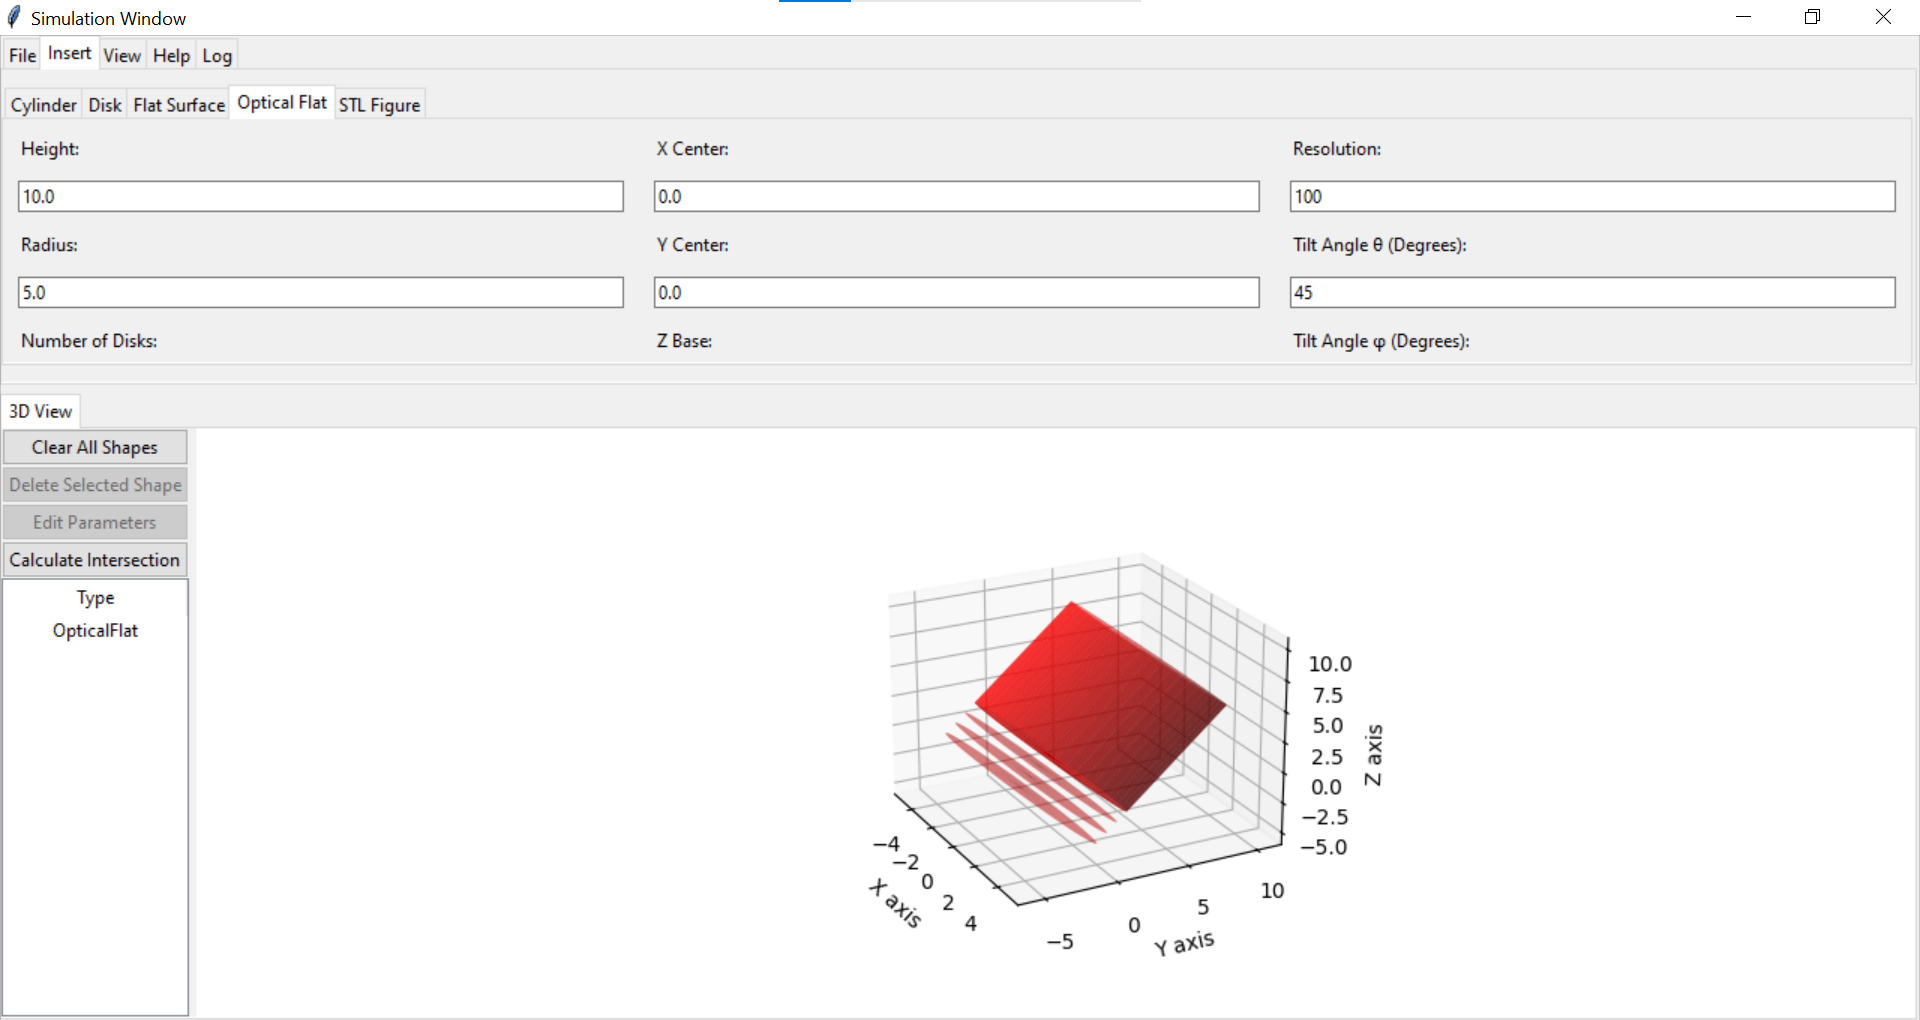
\includegraphics[width=\textwidth]{Images/Appendix/simulation/optical_flat}
\caption{Configuration of an optical flat intersecting with multiple disks at an angle, highlighting the complex intersection capabilities of the tool.}
\end{figure}

\subsection{3D Surface from Height Map Data}
\begin{figure}[H]
\centering
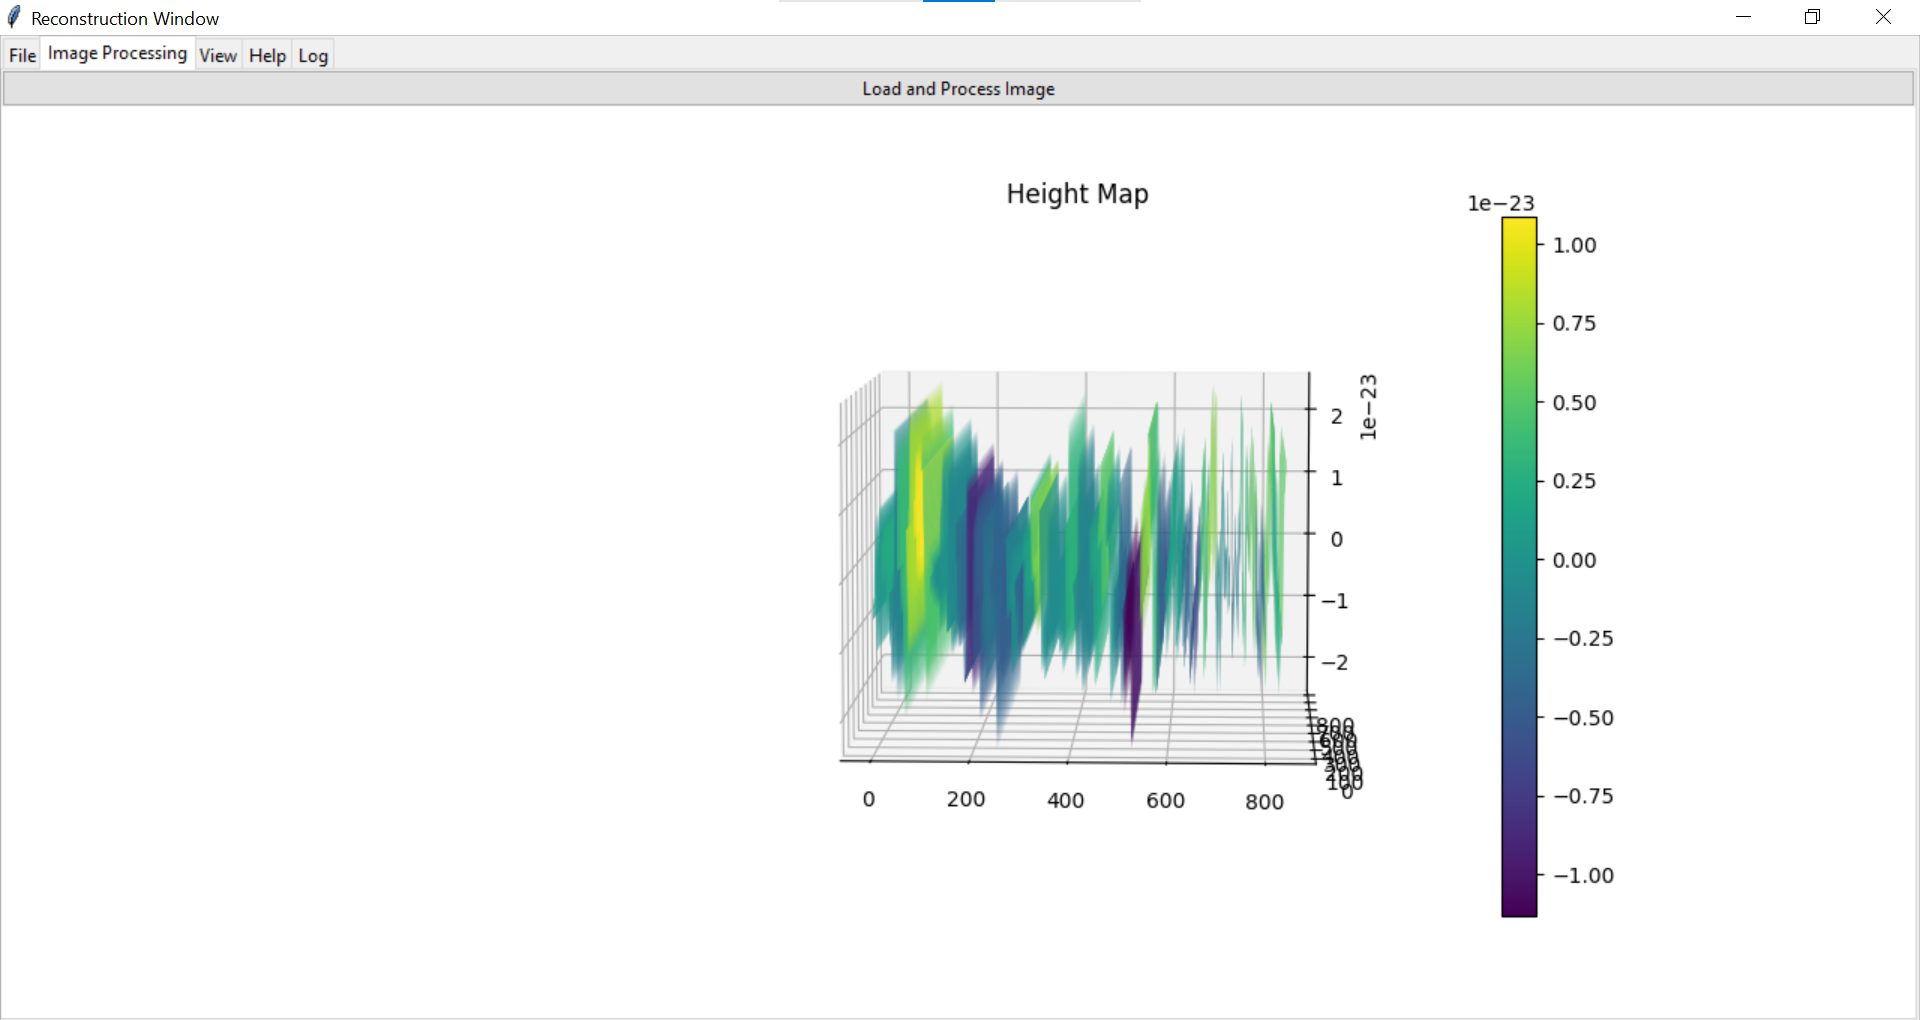
\includegraphics[width=\textwidth]{Images/Appendix/reconstruction/3D_surface}
\caption{3D visualization of a height map converted from image data, showing the application’s ability to render surface topographies.}
\end{figure}

\subsection{Log File Output}
\begin{figure}[H]
\centering
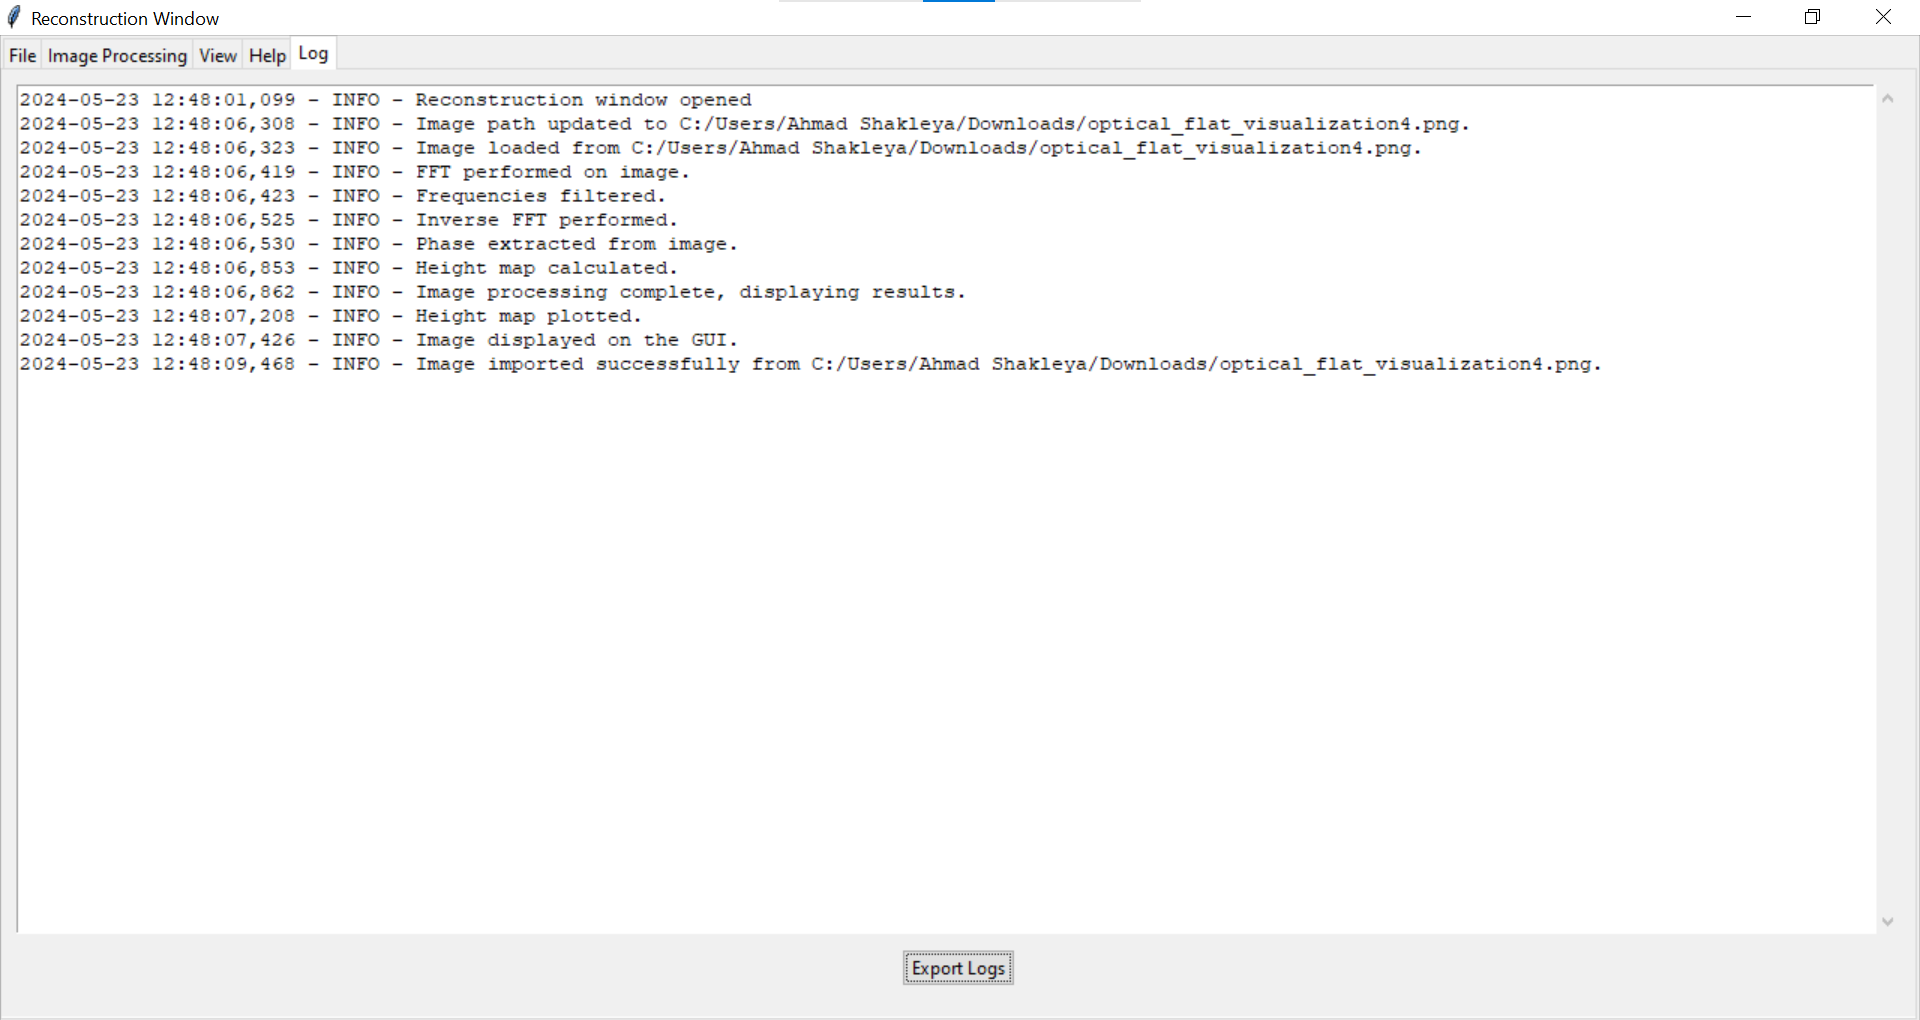
\includegraphics[width=\textwidth]{Images/Appendix/reconstruction/log}
\caption{Log file output of the application capturing various steps such as loading images, processing FFT, and generating height maps.}
\end{figure}

\end{document}
